According to the three-tier architecture, our system will be composed of these high-level components:
\begin{itemize}
    \item Client tier;
    \item Server tier;
    \item Data tier.
\end{itemize}
Now we need to distinguish into the case of the mobile application and the web one. 

\subsubsection{Mobile application}

    \begin{figure}[H]
        \centering
        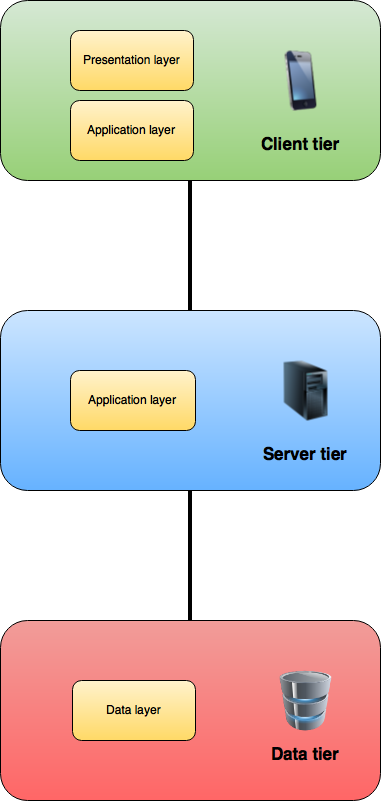
\includegraphics[width=5cm]{./Images/MobileTier.png}
        \caption{Three-tier architecture for the mobile application}
    \end{figure}

    \begin{itemize}
    \item Client tier: it will implement the presentation layer but also the application layer: in fact, the client's device, once it has received from the server XML data or JSON data, has to parse them and then to create the page that will be visualized on the device.
    \item Server tier: it will implement the business logic; this means that this server is in charge to manipulate the data and perform detailed processing. For example, this level will be responsible for managing all the requests from users and changing taxi drivers' status dynamically. 
    \item Data tier: it refers only to the data layer, where all the data of our system will be stored. For example, it will store all the details about requests, taxi drivers' information and so on.
    \end{itemize}

Caso web:
Client tier: presentation layer
Server tier: presentation layer+business layer
Data tier: gestione dati

This means that the presentation layer, the business layer and the data layer will be maintained as separated modules on three different tiers: 
\begin{itemize}
	\item Presentation tier: it will implement the presentation layer which refers to users interfaces. In particular, in our system this layer will run on users' devices (that are provided with our mobile application or web application) and on taxi drivers devices (that are provided with our taxi drivers' application).
\newline
These three tiers have been identified as the main components of our system; so, we will have one high-level component on the clients-side and two referring to the %system-side(???).